% \chapter*{\Huge Big Title Here}
% \addcontentsline{toc}{chapter}{Big Title Here}  % Add to TOC if needed

% \chapter{Components integration - a deep mechanistic approach} % propositions de titre
\chapter{A deep mechanistic model: Grounded mechanistic model for adaptive knowledge}
%----------------------------------------------------------------------------------------
%	SECTION 
%----------------------------------------------------------------------------------------
\section{Introduction}
%-----------%-----------
%	SOUS-SECTION 
%-----------%-----------

 % pour justifier la précision obtenue: Moreover, for BRD and similar conditions there is no universally accepted “gold standard” diagnostic: clinical thresholds vary by practitioner and farm context, and standard laboratory tests (e.g., bacterial culture) can take days to return, further compounding uncertainty in disease classification

\subsection{Contextual background}
Modern sensor modalities (e.g., lung ultrasound, video and audio surveillance, etc) offer high‑frequency, objective measurements that overcome many limitations of human observation (inter‑observer variability, delayed reporting). However, these measurements represent only the observable manifestations of underlying pathophysiological processes and thus provide an incomplete, noisy “snapshot” of disease state—what Yoan Bourhis (2017) aptly describes as the “tip of the iceberg” .

Aleatoric uncertainty refers to the inherent noise and variability present in the data itself. In the context of sensor‑based diagnostics—such as lung ultrasound videos of cattle, aleatoric uncertainty arises from factors beyond the model’s control: image acquisition artifacts, animal movement, inconsistent probe positioning, and intrinsic biological variability in disease presentation. Because aleatoric uncertainty reflects randomness in the observation process, it cannot be reduced simply by collecting more data; instead, it must be explicitly modelled so that downstream predictions correctly reflect the limits of information contained in each measurement. Epistemic uncertainty, by contrast, captures the model’s lack of knowledge about the correct mapping from inputs to outputs. This form of uncertainty is highest when the model encounters examples that are far from the distribution of its training data—rare clinical presentations, novel farm environments, or unforeseen sensor configurations. Unlike aleatoric uncertainty, epistemic uncertainty can be reduced through the acquisition of additional, representative training examples. Crucially, a model can output a high softmax score (traditional logits interpreted as probabilities) even when its epistemic uncertainty is large, leading to overconfident and potentially erroneous predictions \cite{gal_dropout_2016}.

Epidemiological forecasting relies on mechanistic models, which codify known biological relationships (transmission rates, immune response kinetics, within‑host pathogen dynamics) into mathematically tractable systems of equations. While these models capture long‑term disease trajectories and can simulate the effects of interventions at the population level, they are poorly informed by sensor data when observations are unstructured, sparse and noisy.


% Standard deep‑learning pipelines commonly equate the softmax output of the final layer with predictive confidence, yet this conflation masks both aleatoric and epistemic uncertainties and gives no indication of when a prediction should be trusted. In high‑stakes veterinary diagnostics, such overconfidence can result in inappropriate treatments, delayed intervention, and significant economic and welfare costs.


%-----------%-----------
%	SOUS-SECTION 
%-----------%-----------
\subsection{Article Originality and objectives}

\paragraph{To what extent can automated short-term diagnostics derived from limited sensor observations effectively inform and specify a mechanistic epidemiological model for long-term disease prognosis?} In this work, we propose and explore a novel hybrid methodology explicitly aimed at integrating deep learning, sensor-based diagnostics with a mechanistic epidemiological model (Fig \ref{fig:chap4-question1}). Specifically, we develop an approach that leverages short-term, sensor-derived diagnostics obtained from limited Lung Ultrasound (LUS) video data to inform parameter calibration in epidemiological models. We employ a Bayesian Deep Mechanistic approach to bridge sensor-based diagnostics and mechanistic forecasting. This integration aims to enhance the interpretability, and practical applicability of epidemiological prognosis, enabling accurate long-term disease management strategies from inherently limited and uncertain short-term observations. 


\begin{figure}[H]
  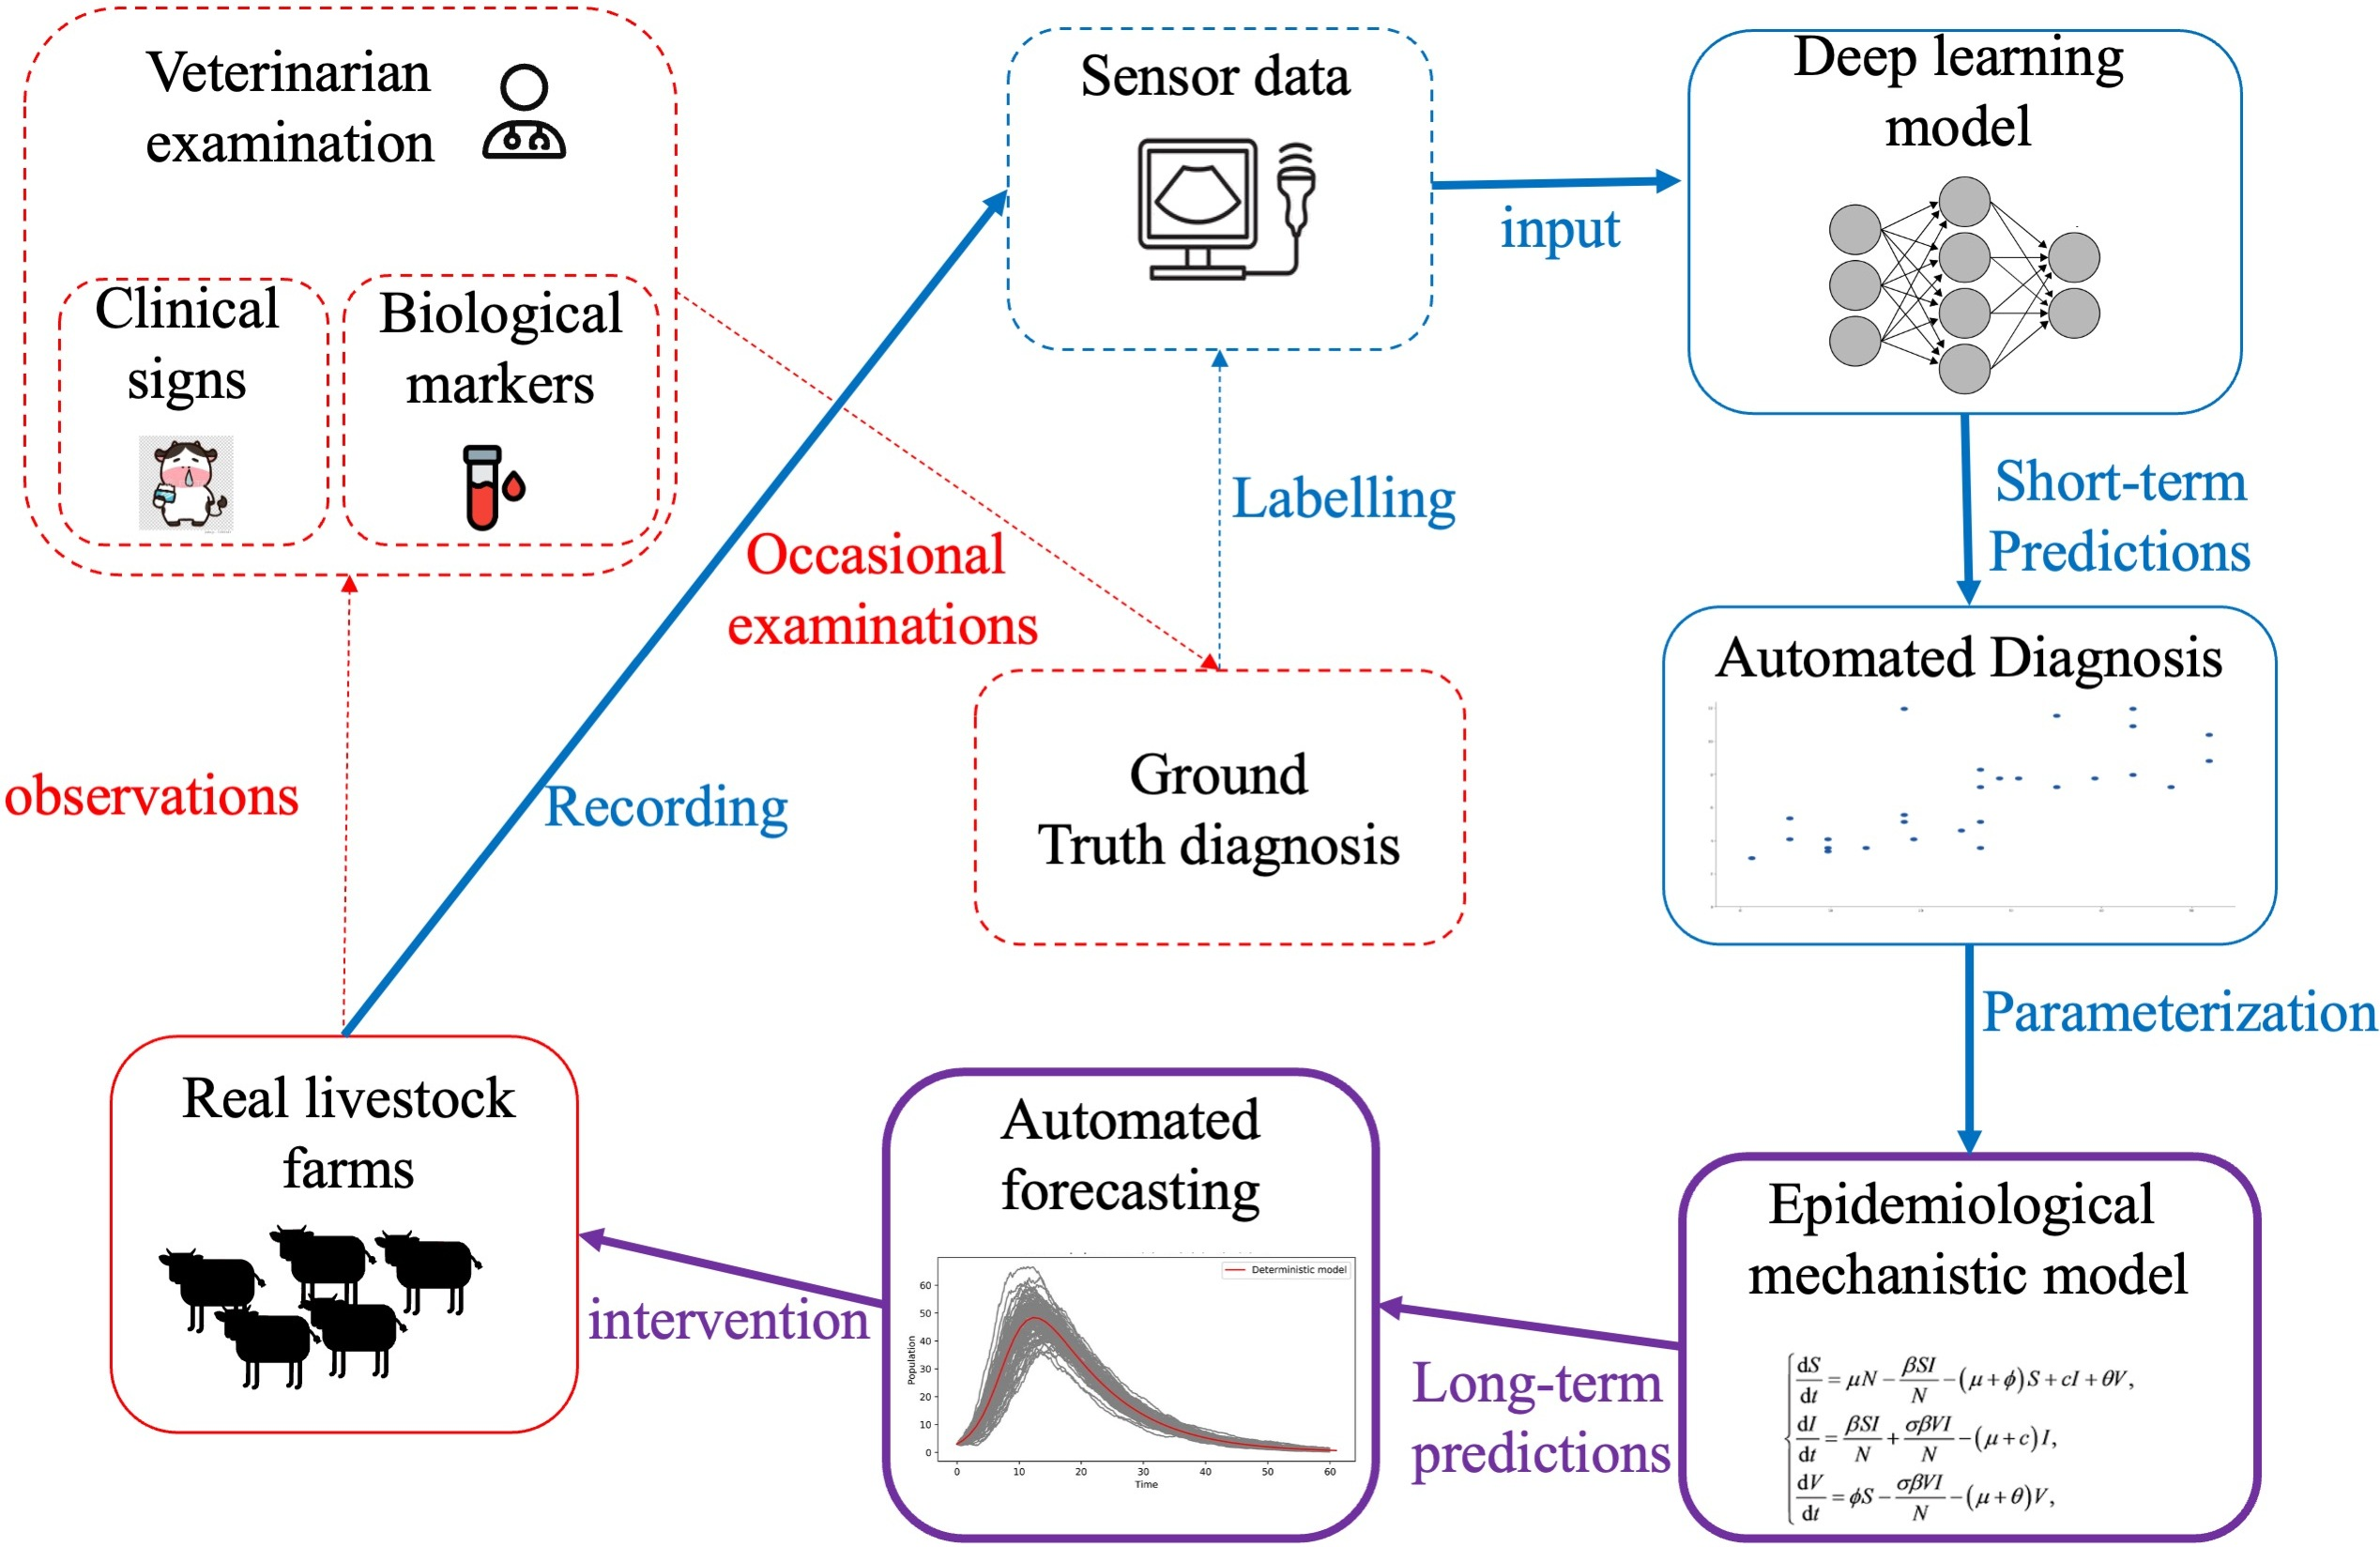
\includegraphics[width=\linewidth]{figures/chap4/chap4-question1.jpg}
  \caption{Sketch workflow of a ...}
  \label{fig:chap4-question1}
\end{figure}

\paragraph{How can intrinsic uncertainties inherent in sensor-derived diagnostic data, especially noisy observations such as Lung Ultrasound (LUS) videos, be explicitly quantified and incorporated into mechanistic models to ensure a more robust and trustworthy prognostic prediction ?}

Given the intrinsic uncertainty and noisiness of real-world LUS videos, exacerbated by animal movement and image acquisition limitations, this work explicitly addresses the quantification and integration of these uncertainties into the diagnostic and prognostic pipeline. We variational methods in Bayesian deep learning model to quantify the uncertainty associated with sensor-based diagnostic predictions. Bayesian probability theory offers us mathematically grounded tools to reason about model uncertainty. These quantified uncertainties are subsequently managed through two complementary approaches: either by filtering out high-uncertainty, unreliable observations (Out-of-distribution detection) to ensure safe prognosis and prioritize them for detailed veterinary reassessment, or by directly propagating uncertainties into mechanistic model calibration through uncertainty-weighted parameter inference. This dual strategy enhances the robustness, reliability, and practical applicability of long-term prognostic predictions.


%-----------%-----------
%	SOUS-SECTION 
%-----------%-----------
\subsection{Main contributions}
This chapter introduces the Bayesian Deep Mechanistic (BDM) model, a novel integrative approach that leverages both data-driven diagnostics derived from sensor technologies and knowledge-driven epidemiological modeling. This integration addresses critical limitations inherent in existing diagnostic and prognostic methodologies, specifically for Bovine Respiratory Disease (BRD), by explicitly quantifying and managing uncertainty from limited and noisy sensor observations. Three main contributions emerge from the approach presented in this chapter:


\begin{enumerate}
    \item \textbf{Coupling punctual diagnostics with mechanistic forecasting (fig \ref{fig:chap4-method1}).}   We designed and trained a hybrid deep learning pipeline, a spatio-temporal CNN‑RNN—that ingests raw lung ultrasound (LUS) video clips and outputs a binary infectious status (infectious vs. non‑infectious) for individual bovine. Our dataset comprised 265 LUS videos collected from 163 animals across nine French farms, capturing real‑world variability in lesion appearance, probe positioning, and animal movement.  Crucially, these “punctual” diagnostic predictions served not only as standalone classifiers but also as the empirical anchor for calibrating a mechanistic epidemiological model via Approximate Bayesian Computation (ABC). In practice, we treat each deep learning prediction as a point estimate of batch‑level infection prevalence at discrete observation times; ABC then infers the three key parameters—initial prevalence, average infectious duration, and transmission rate—that best reconcile the mechanistic model’s simulated infection trajectories with these sensor‑derived snapshots. This coupling bridges short‑term, deep learning diagnostics and long‑term, mechanistic forecasts. 

    Although fully automated and practical for on‑farm use, our diagnostic model achieved a relative root‑mean‑square error (RRMSE) of 39\% against veterinarian‑confirmed labels, reflecting the inherent noise and variability of LUS data. When these predictions alone were used to parametrize the mechanistic model, the resulting 30‑day forecast exhibited an RRMSE of 38.4\%, substantially higher than the 23\% error attained when using veterinarian ground‑truth diagnostics. This gap underscores both the promise of automated sensing for scalable disease surveillance and the imperative of explicitly quantifying and managing uncertainty in order to approach the accuracy of expert‑driven prognostics.

    \begin{figure}[H]
      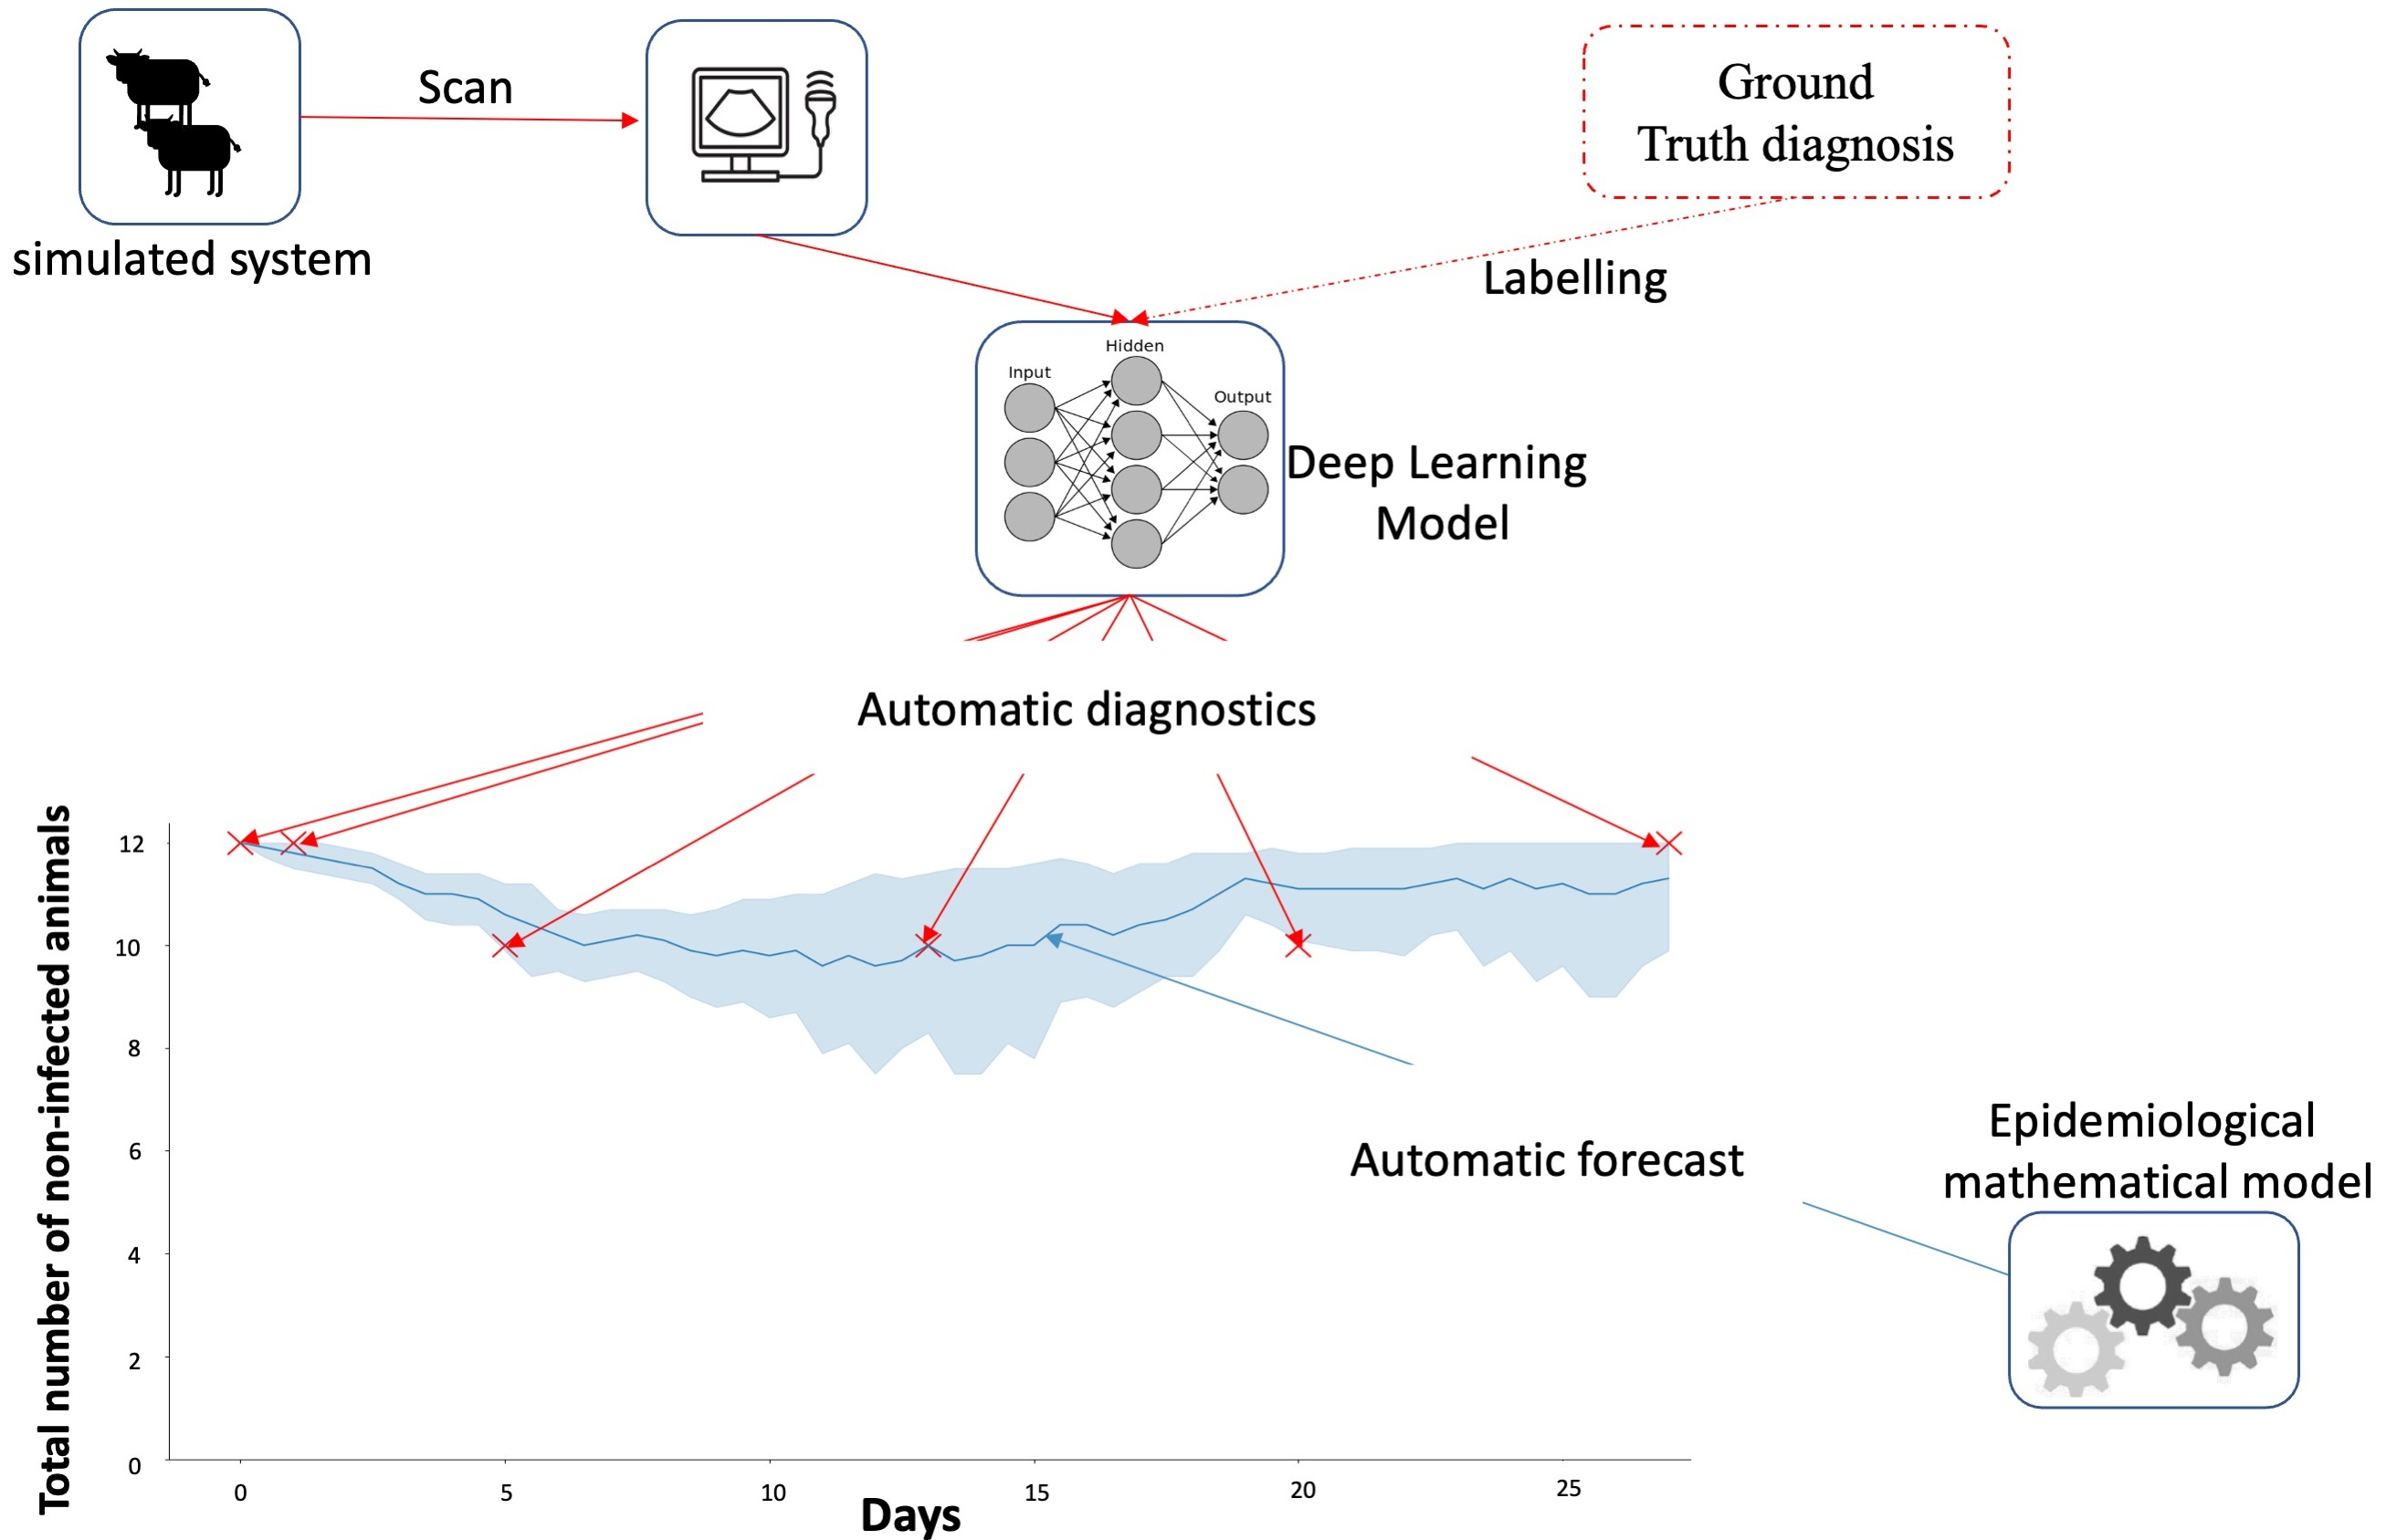
\includegraphics[width=\linewidth]{figures/chap4/method 1.jpg}
      \caption{coupling punctual diagnostics with mechanistic forecasting}
      \label{fig:chap4-method1}
    \end{figure}

    \item \textbf{Sensor observation cleansing through Uncertainty-Based Filtering (fig \ref{fig:chap4-method2}).} Lung ultrasound (LUS) videos are full with sources of noise, animal motion, suboptimal probe positioning, uninterpretable image artifacts—that can lead a deterministic classifier to make confidently wrong predictions (In chapter 1 \ref{fig:chap2-question1},  we achieved only a 72\% accuracy, for a binary classifier, that is low). In order to control this risk in observations used, we had to explicitly capture the epistemic uncertainty (i.e., the model’s lack of knowledge). For that we converted our CNN‑RNN DL model into a Bayesian deep learning model using Monte Carlo Dropout (MCD). During inference, MCD performs dozens of stochastic forward passes with dropout active, producing a distribution of softmax probability vectors rather than a single point estimate. We then quantify uncertainty by computing the Shannon entropy of each video’s averaged class probability distribution—a well‑established acquisition function in active learning that measures the spread (disorder) of predictive beliefs. High entropy indicates low confidence and signals inputs for which the model’s knowledge is insufficient.

    By ranking predictions by entropy, we implemented an uncertainty‑based filter: low‑entropy (high‑confidence) cases are accepted as automatic diagnoses, while high‑entropy (low‑confidence) cases are flagged for veterinarian review. This selective acceptance dramatically improved diagnostic accuracy, lowering the relative root‑mean‑square error (RRMSE) from 39\% (deterministic predictions) to 32\% against veterinarian ground truth. Crucially, when only filtered (high‑confidence) diagnoses were used to calibrate our epidemiological model, the 30‑day forecast error fell to 27.2\% RRMSE—much closer to the 23\% error achieved using full veterinarian diagnoses
    
        \begin{figure}[H]
          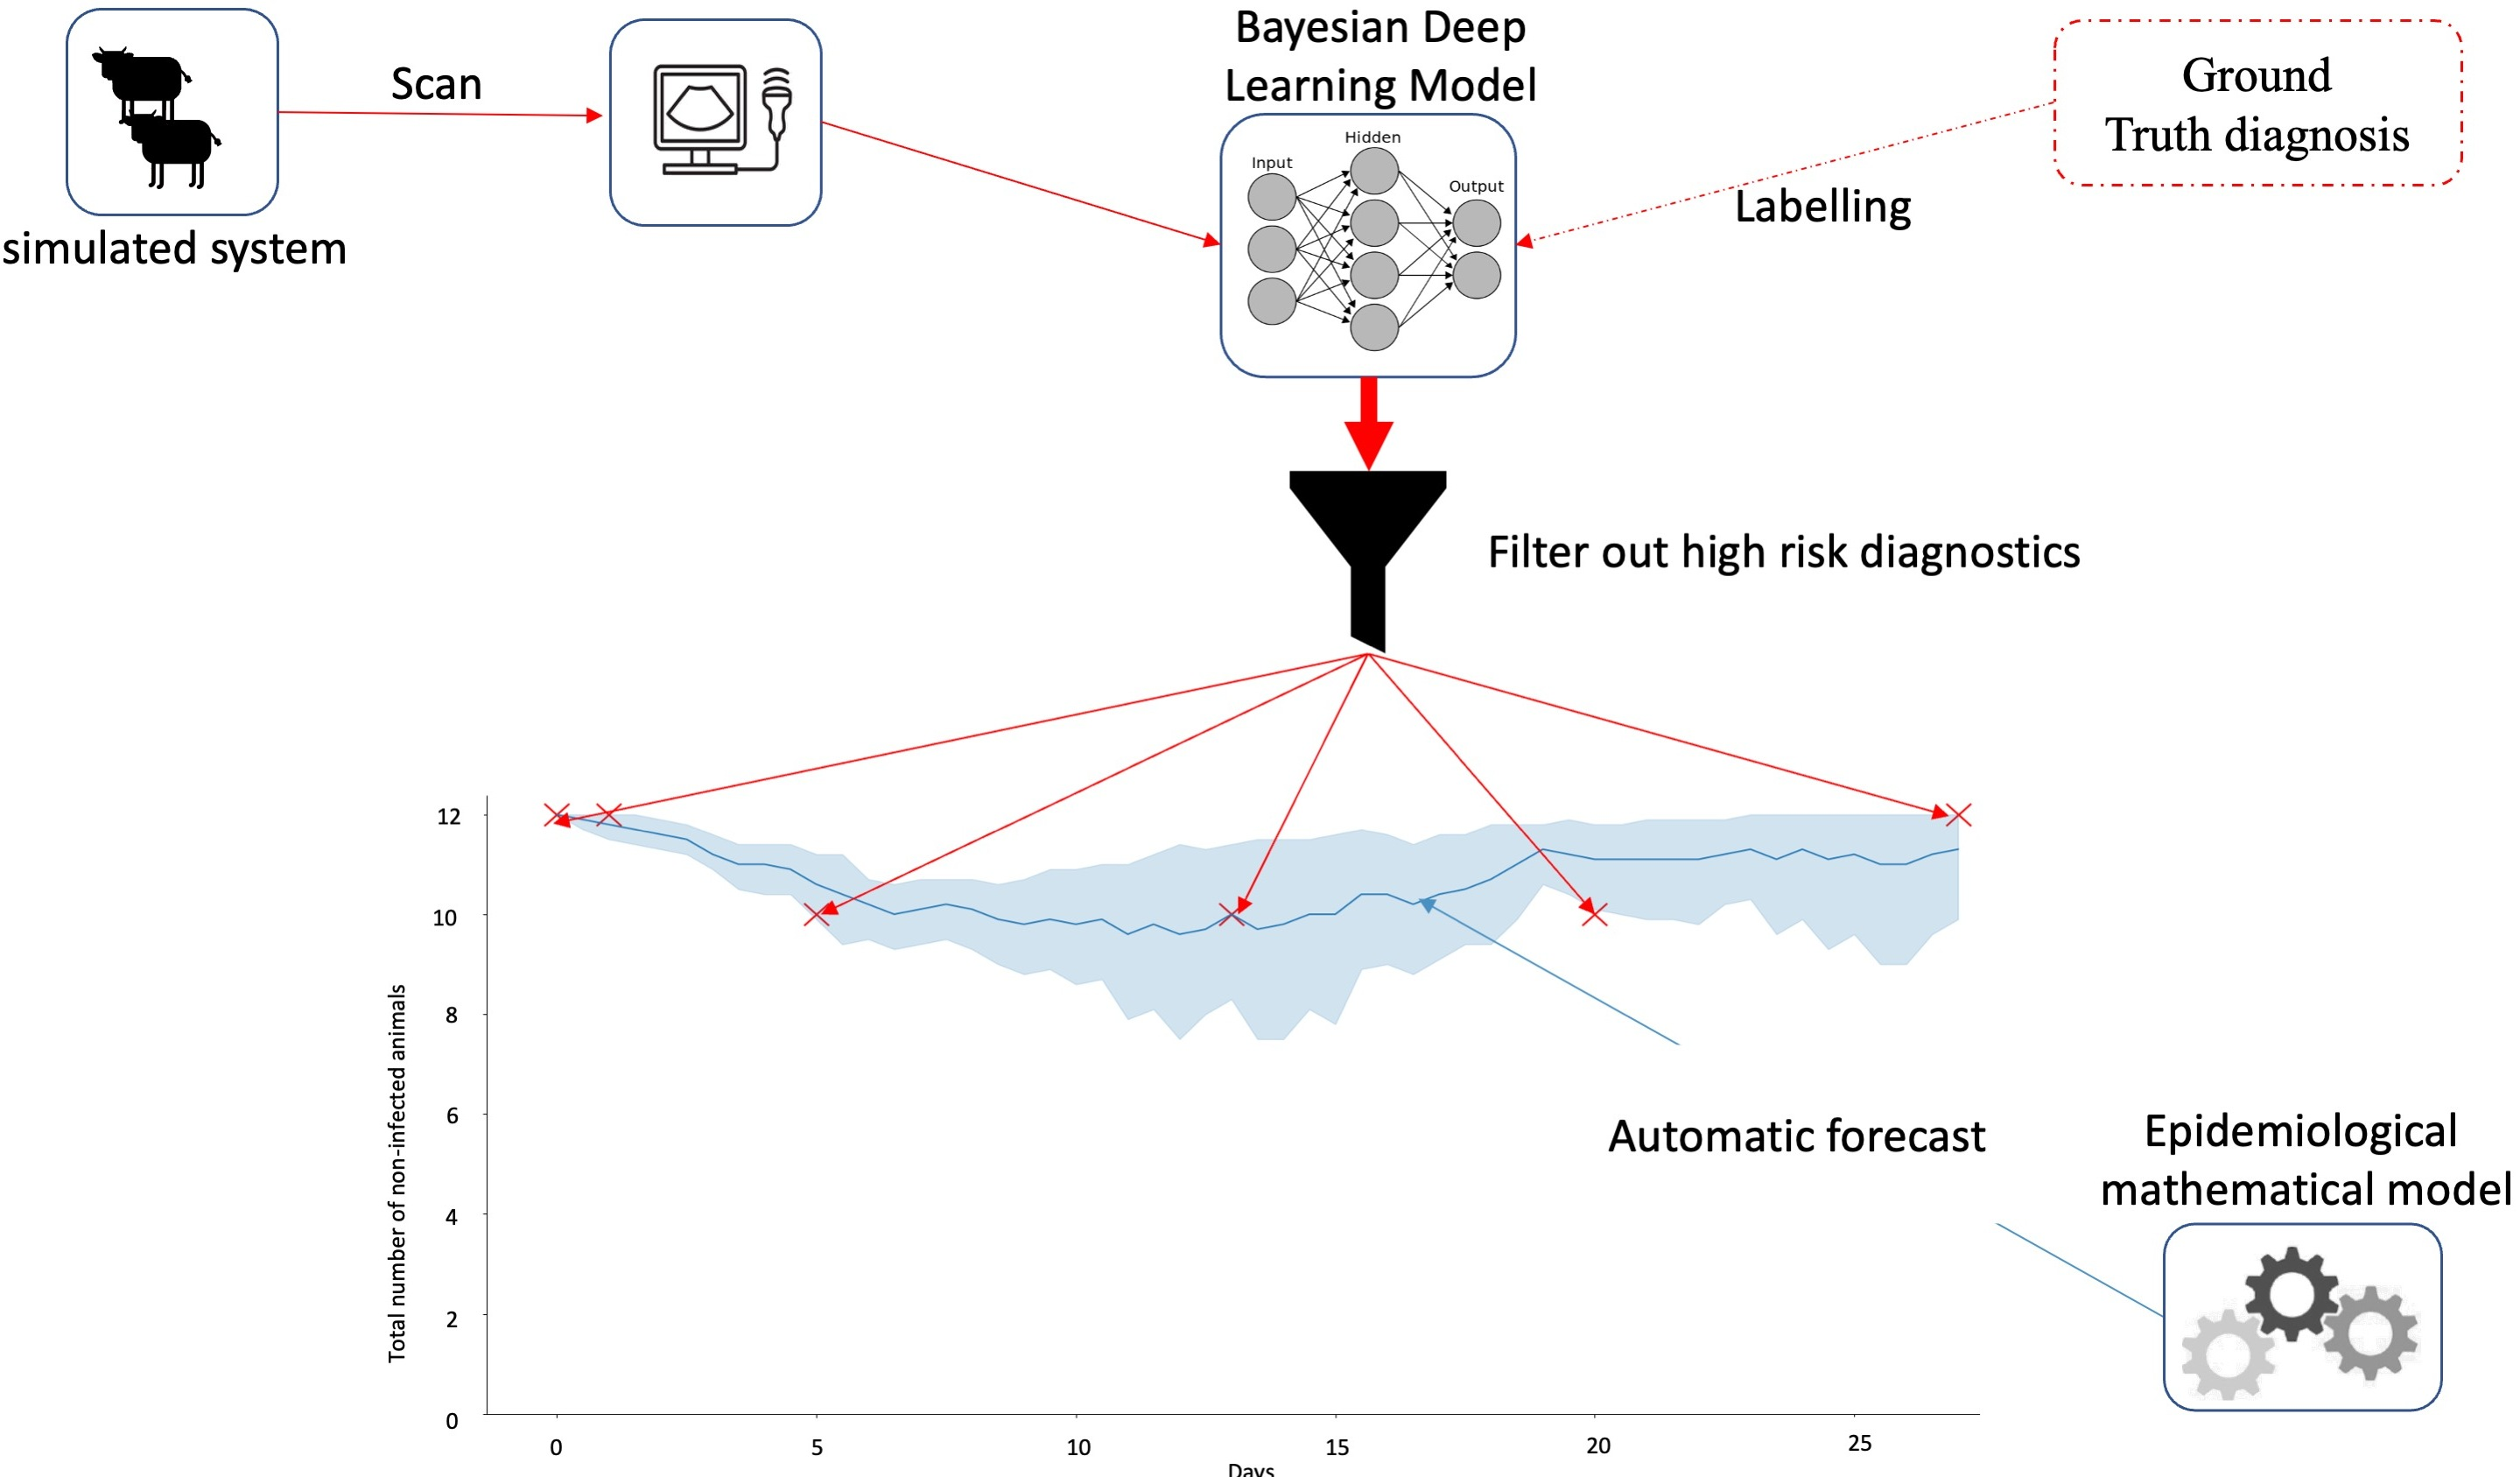
\includegraphics[width=\linewidth]{figures/chap4/method 2.jpg}
          \caption{Sensor observation cleansing through Uncertainty-Based Filtering}
          \label{fig:chap4-method2}
        \end{figure}

    \item \textbf{Prognosis robustness through Uncertainty Propagation (fig \ref{fig:chap4-method3}).} Rather than discarding low‑confidence diagnoses, we leveraged each prediction’s quantified uncertainty to inform the parametrization of a stochastic mechanistic epidemiological model. After obtaining a posterior distribution (uncertainties) over batch‑level infectious counts via Monte Carlo Dropout, we extracted both the mean (as the point estimate of infected prevalence) and its variance (as a measure of diagnostic confidence). During Approximate Bayesian Computation (ABC) parameter inference, we replaced the standard Euclidean distance with a weighted version in which each observation’s contribution was inversely proportional to its uncertainty (i.e., higher variance → lower weight). This uncertainty‑weighted inference ensures that reliable, low‑variance diagnostics exert greater influence on parameter estimation (pathogen transmission rate, mean duration in the infectious state, mean duration in the pre-infectious state), while noisy, high‑variance observations contribute less, effectively down-weighting potentially misleading observations rather than excluding it outright. The result is a more robust posterior over epidemiological parameters and, consequently, more accurate long‑term forecasts: the uncertainty‑propagated model achieved a 30‑day forecast RRMSE of 27.2\% nearly matching the 23\% error obtained when calibrating solely on veterinarian‑confirmed diagnoses. This method also reduces diagnostic error from the deterministic model’s 39\% RRMSE to 32\% RRMSE, matching the improvement seen in our uncertainty‑filtering approach

    These results demonstrate that explicitly propagating diagnostic uncertainty not only improves automated classification but also closes most of the remaining gap between sensor‑based forecasts and expert‑driven prognostics, unlocking robust long‑term predictions from inherently noisy, limited observations. By embedding predictive uncertainty directly into the model calibration process, our approach preserves information from all sensor‑based observations maximizing data utility, while mitigating the impact of noise.

    \begin{figure}[H]
      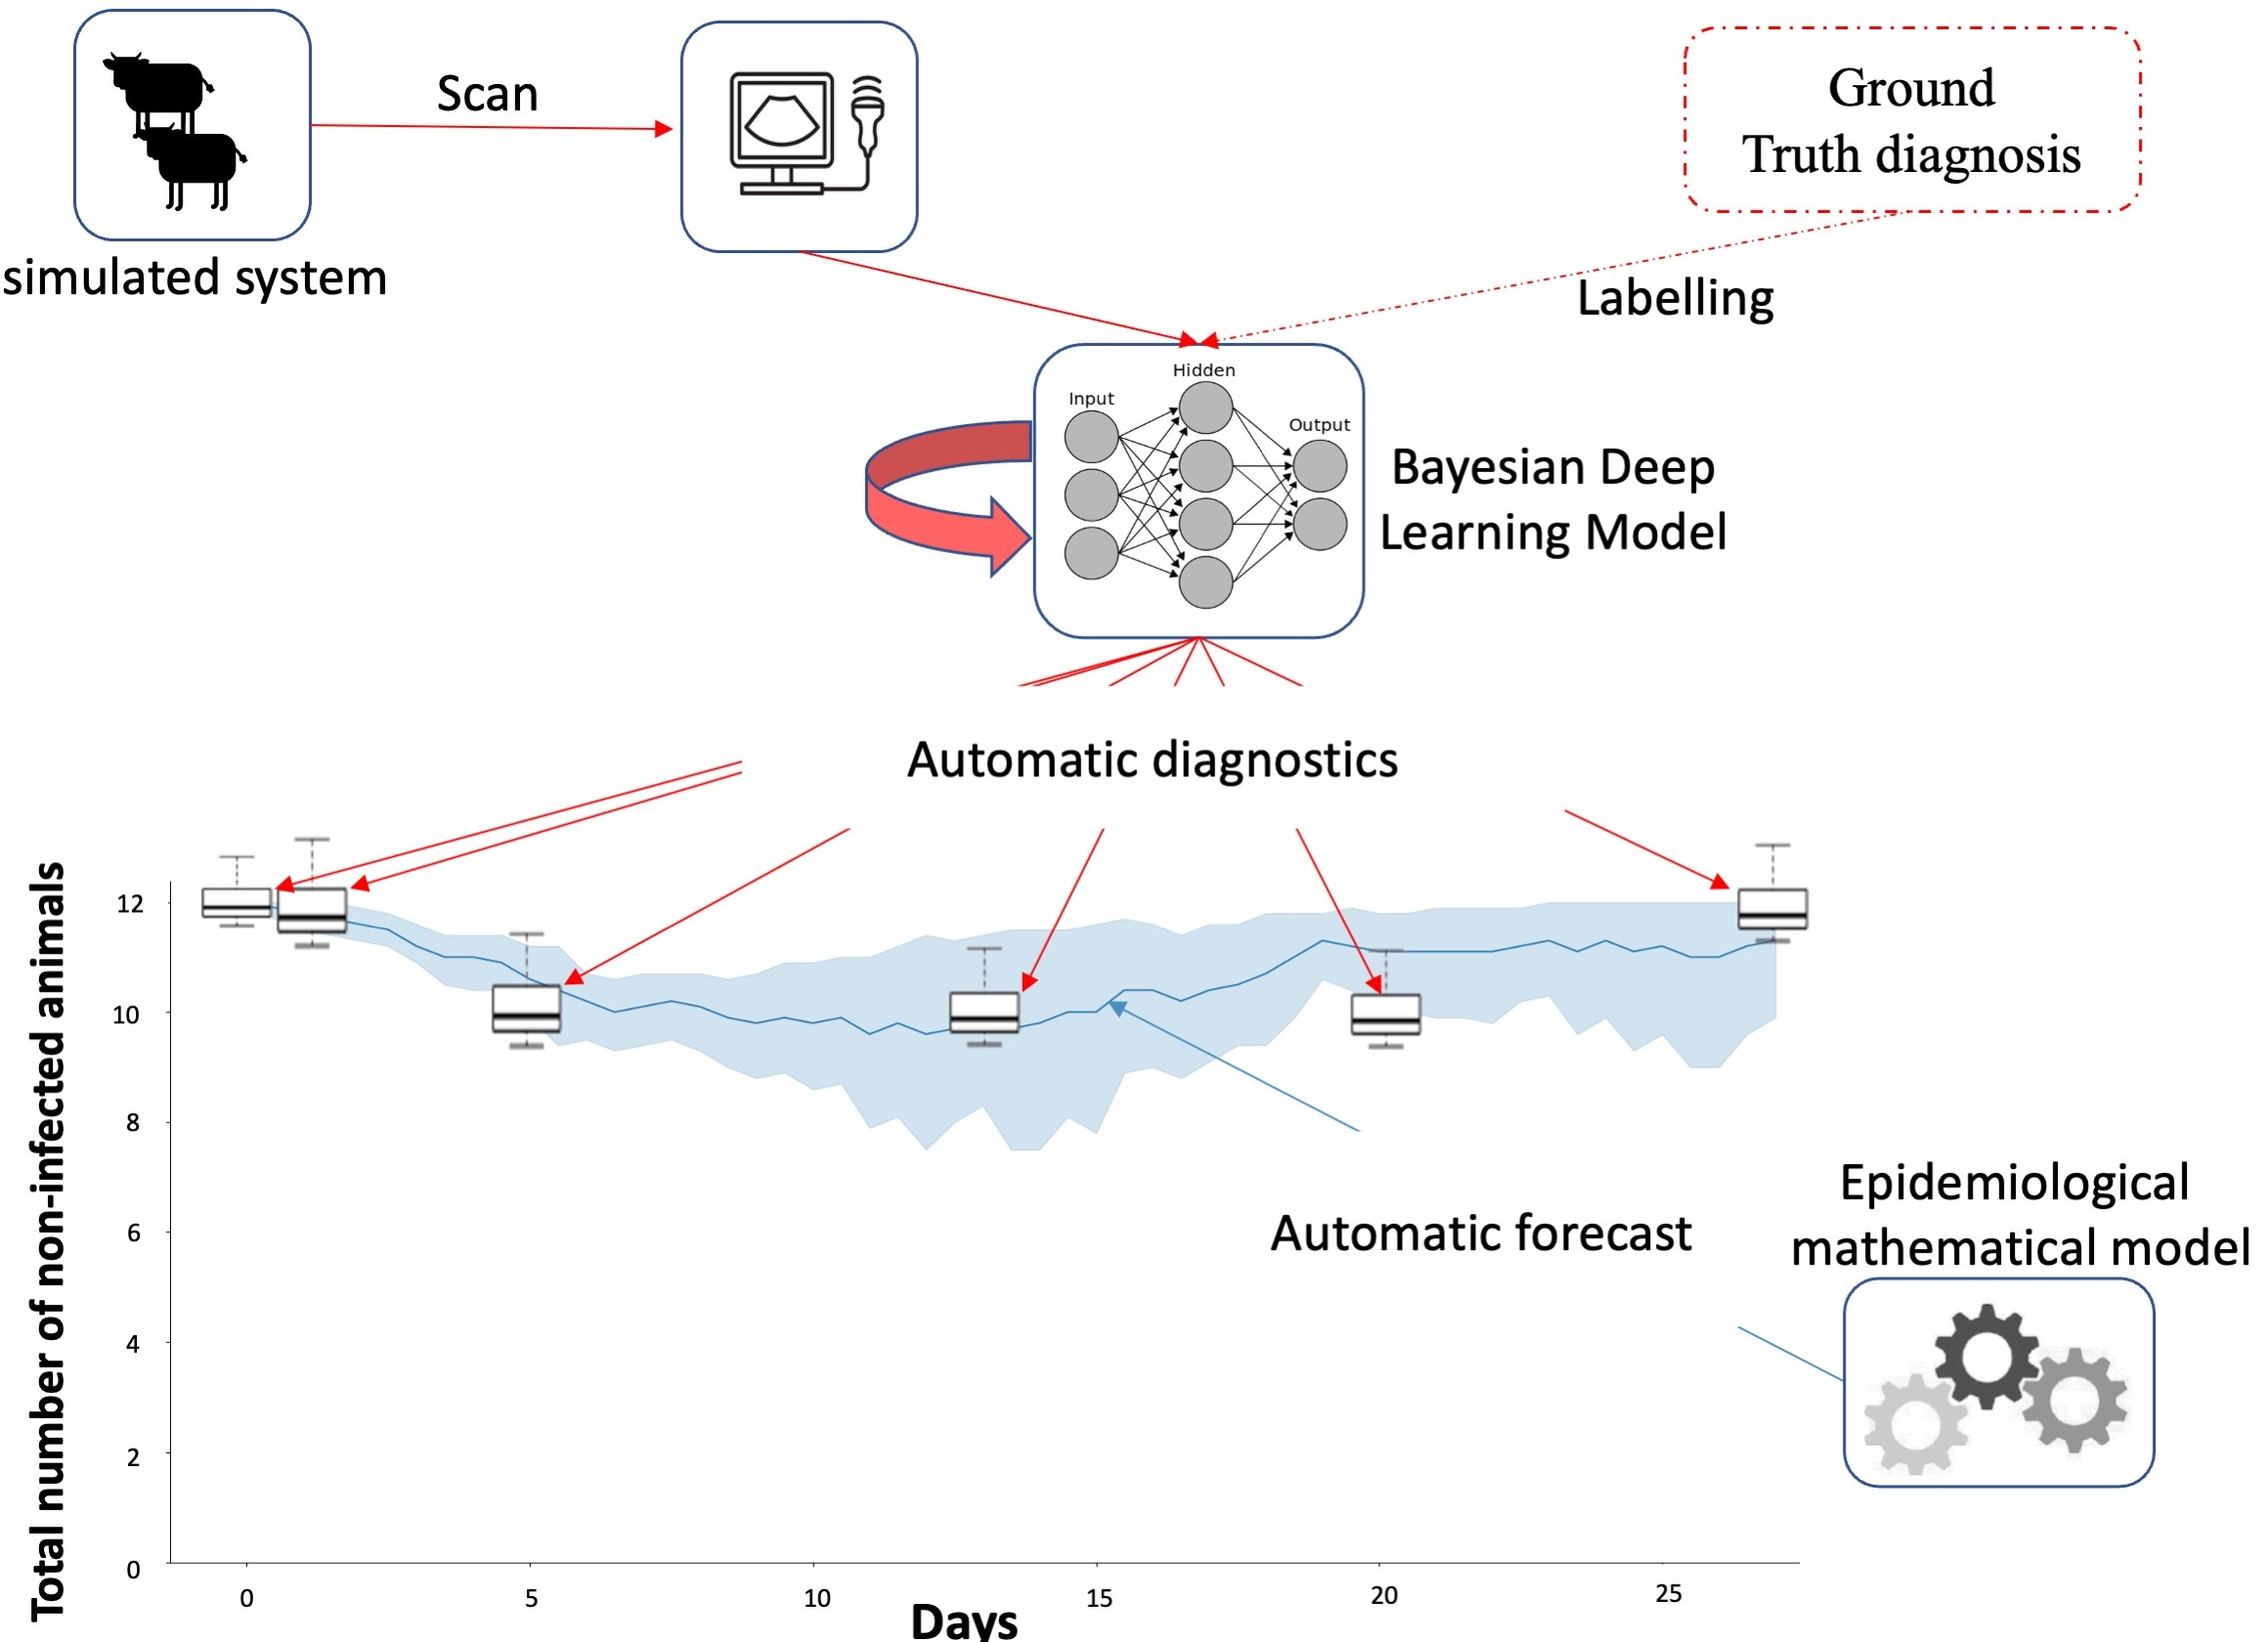
\includegraphics[width=\linewidth]{figures/chap4/method 3.jpg}
      \caption{Prognosis robustness through Uncertainty Propagation}
      \label{fig:chap4-method3}
    \end{figure}
    
\end{enumerate}

 
\subsection{[In French] Résumé grand public} 
La santé animale et la prévention des maladies infectieuses reposent de plus en plus sur des technologies de diagnostic automatisées, comme l’échographie pulmonaire chez les bovins. Toutefois, ces données issues de capteurs sont souvent bruyantes, incomplètes et sujettes à des erreurs d’interprétation. Notre étude propose une nouvelle approche hybride qui combine l’intelligence artificielle (IA) et les modèles mathématiques traditionnels (appelés «mécanistiques») pour améliorer la détection précoce et la prévision à long terme de la maladie respiratoire bovine.

Nous avons d’abord développé un modèle d’apprentissage profond capable d’analyser automatiquement de courtes vidéos d’échographie pulmonaire et de prédire si un animal est infectieux ou non. Pour tenir compte de l’incertitude inhérente à ces diagnostics automatisés (problèmes de qualité d’image, mouvements de l’animal…), nous utilisons une technique bayésienne qui mesure la confiance de chaque prédiction. Les cas où le modèle est peu sûr sont soit signalés pour un examen vétérinaire, soit pondérés de façon moindre dans les étapes suivantes.

Ensuite, ces diagnostics ponctuels, enrichis de leur degré de confiance, servent à calibrer un modèle épidémiologique mathématique qui simule la propagation de la maladie dans un troupeau sur plusieurs semaines. Cette intégration «fusion» permet de produire des prévisions de l’évolution de l’infection plus fiables que celles basées uniquement sur l’IA ou uniquement sur les modèles traditionnels. Concrètement, notre méthode réduit l’erreur de prédiction à 27\% sur 30 jours — un résultat proche de la précision obtenue lorsqu’on utilise exclusivement des diagnostics vétérinaires, mais avec un processus entièrement automatisé et évolutif pour une utilisation directe en élevage.

En résumé, cette étude démontre qu’il est possible d’exploiter efficacement des données de capteurs imparfaites grâce à une modélisation hybride : l’intelligence artificielle apporte une analyse rapide et à grande échelle, tandis que le modèle mathématique garantit une prévision robuste à long terme. Cette approche ouvre la voie à une surveillance de la santé animale plus précise, proactive et accessible, contribuant à améliorer le bien‑être des animaux et à réduire les pertes économiques liées aux maladies infectieuses.


\section{Article published in Preventive Veterinary Medicine (Elsevier), 2024}


    % \input{chapters/chap1-article} # pas besoin de mettre un file appart sauf si j'ai des choses spécifiques à rajouter pour cette partie
    \includepdf[pages=-]{articles/PVM.pdf}  % Replace with your actual filename

